% This is "sig-alternate.tex" V2.1 April 2013
% This file should be compiled with V2.5 of "sig-alternate.cls" May 2012
%
% This example file demonstrates the use of the 'sig-alternate.cls'
% V2.5 LaTeX2e document class file. It is for those submitting
% articles to ACM Conference Proceedings WHO DO NOT WISH TO
% STRICTLY ADHERE TO THE SIGS (PUBS-BOARD-ENDORSED) STYLE.
% The 'sig-alternate.cls' file will produce a similar-looking,
% albeit, 'tighter' paper resulting in, invariably, fewer pages.
%
% ----------------------------------------------------------------------------------------------------------------
% This .tex file (and associated .cls V2.5) produces:
%       1) The Permission Statement
%       2) The Conference (location) Info information
%       3) The Copyright Line with ACM data
%       4) NO page numbers
%
% as against the acm_proc_article-sp.cls file which
% DOES NOT produce 1) thru' 3) above.
%
% Using 'sig-alternate.cls' you have control, however, from within
% the source .tex file, over both the CopyrightYear
% (defaulted to 200X) and the ACM Copyright Data
% (defaulted to X-XXXXX-XX-X/XX/XX).
% e.g.
% \CopyrightYear{2007} will cause 2007 to appear in the copyright line.
% \crdata{0-12345-67-8/90/12} will cause 0-12345-67-8/90/12 to appear in the copyright line.
%
% ---------------------------------------------------------------------------------------------------------------
% This .tex source is an example which *does* use
% the .bib file (from which the .bbl file % is produced).
% REMEMBER HOWEVER: After having produced the .bbl file,
% and prior to final submission, you *NEED* to 'insert'
% your .bbl file into your source .tex file so as to provide
% ONE 'self-contained' source file.
%
% ================= IF YOU HAVE QUESTIONS =======================
% Questions regarding the SIGS styles, SIGS policies and
% procedures, Conferences etc. should be sent to
% Adrienne Griscti (griscti@acm.org)
%
% Technical questions _only_ to
% Gerald Murray (murray@hq.acm.org)
% ===============================================================
%
% For tracking purposes - this is V2.0 - May 2012

\documentclass{sig-alternate-05-2015}




\usepackage{times}
\usepackage{CJKutf8}
\usepackage{mathrsfs}
\usepackage{textcomp}
\usepackage{verbatim}
\usepackage{amsmath}
\usepackage{amsfonts}
\usepackage{xspace}
\usepackage{xcolor}
\usepackage{url}
\usepackage{balance}
\usepackage{booktabs}
\usepackage{multirow}
\usepackage{rotating}
\usepackage{fancyvrb}
\usepackage{lastpage}
\usepackage{alltt}
\usepackage{etoolbox}
\usepackage{cleveref} % After hyperref, listings
\usepackage{fancyhdr}
\usepackage{listings}

\usepackage{caption}
\usepackage{subcaption}

\usepackage{tikz}
\usetikzlibrary{shapes,snakes}


\usepackage{amsmath}
\usepackage{amssymb}
\usepackage{wasysym}

%The given symbol or text (\text{mytext}) in a circle
%To be used always in math mode
\newcommand{\circlesign}[1]{ 
    \mathbin{
        \mathchoice
        {\buildcirclesign{\displaystyle}{#1}}
        {\buildcirclesign{\textstyle}{#1}}
        {\buildcirclesign{\scriptstyle}{#1}}
        {\buildcirclesign{\scriptscriptstyle}{#1}}
    } 
}


\newcommand\buildcirclesign[2]{%
    \begin{tikzpicture}[baseline=(X.base), inner sep=0, outer sep=0]
    \node[draw,circle] (X)  {\ensuremath{#1 #2}};
    \end{tikzpicture}%
}

\definecolor{lbcolor}{rgb}{0.9,0.9,0.9}
\lstset{
    tabsize=2,    
    language=C,
    basicstyle=\footnotesize\ttfamily,
    upquote=true,
    aboveskip={1.5\baselineskip},
    columns=fixed,
    extendedchars=false,
    showtabs=false,
    showspaces=false,
    showstringspaces=false,
    identifierstyle=\ttfamily,
    keywordstyle=\color[rgb]{0,0,1},
    commentstyle=\color[rgb]{0.026,0.112,0.095},
    stringstyle=\color[rgb]{0.627,0.126,0.941},
    numberstyle=\color[rgb]{0.205, 0.142, 0.73},
}


\usepackage{macro}
\newenvironment{CompactItemize}{\begin{itemize}}{\end{itemize}}
\def\code#1{{\texttt{#1}}}


\usepackage{colorhist}
 
\usepackage{minted}



\begin{document}

% Copyright
\setcopyright{acmcopyright}
%\setcopyright{acmlicensed}
%\setcopyright{rightsretained}
%\setcopyright{usgov}
%\setcopyright{usgovmixed}
%\setcopyright{cagov}
%\setcopyright{cagovmixed}


% DOI
\doi{XX.XXX/XXX_X}

% ISBN
\isbn{XX}

%Conference
\conferenceinfo{XXXXX}{XXXX, 2013, XX, XX, XXX}

\acmPrice{\$15.00}

%
% --- Author Metadata here ---
\conferenceinfo{XXXXX}{'XXXX', USA}
%\CopyrightYear{2007} % Allows default copyright year (20XX) to be over-ridden - IF NEED BE.
%\crdata{0-12345-67-8/90/01}  % Allows default copyright data (0-89791-88-6/97/05) to be over-ridden - IF NEED BE.
% --- End of Author Metadata ---

\title{Docker Container-based Scalable Partitioning for Apache Spark
Scale-Up Server Scalability}
%\subtitle{[Extended Abstract]
%\titlenote{A full version of this paper is available as
%\textit{Author's Guide to Preparing ACM SIG Proceedings Using
%\LaTeX$2_\epsilon$\ and BibTeX} at
%\texttt{www.acm.org/eaddress.htm}}}
%
% You need the command \numberofauthors to handle the 'placement
% and alignment' of the authors beneath the title.
%
% For aesthetic reasons, we recommend 'three authors at a time'
% i.e. three 'name/affiliation blocks' be placed beneath the title.
%
% NOTE: You are NOT restricted in how many 'rows' of
% "name/affiliations" may appear. We just ask that you restrict
% the number of 'columns' to three.
%
% Because of the available 'opening page real-estate'
% we ask you to refrain from putting more than six authors
% (two rows with three columns) beneath the article title.
% More than six makes the first-page appear very cluttered indeed.
%
% Use the \alignauthor commands to handle the names
% and affiliations for an 'aesthetic maximum' of six authors.
% Add names, affiliations, addresses for
% the seventh etc. author(s) as the argument for the
% \additionalauthors command.
% These 'additional authors' will be output/set for you
% without further effort on your part as the last section in
% the body of your article BEFORE References or any Appendices.



% Just remember to make sure that the TOTAL number of authors
% is the number that will appear on the first page PLUS the
% number that will appear in the \additionalauthors section.

\maketitle


%한글 버전으로 출력 하고 싶으면, korture를 Enable 해주시고, korefalse를 주석 처리 해주세요.
\newif\ifkor
\kortrue 
%\korfalse

\begin{abstract}
This paper provides a sample of a \LaTeX\ document which conforms,
somewhat loosely, to the formatting guidelines for
ACM SIG Proceedings. It is an {\em alternate} style which produces
a {\em tighter-looking} paper and was designed in response to
concerns expressed, by authors, over page-budgets.
It complements the document \textit{Author's (Alternate) Guide to
Preparing ACM SIG Proceedings Using \LaTeX$2_\epsilon$\ and Bib\TeX}.
This source file has been written with the intention of being
compiled under \LaTeX$2_\epsilon$\ and BibTeX.

The developers have tried to include every imaginable sort
of ``bells and whistles", such as a subtitle, footnotes on
title, subtitle and authors, as well as in the text, and
every optional component (e.g. Acknowledgments, Additional
Authors, Appendices), not to mention examples of
equations, theorems, tables and figures.

To make best use of this sample document, run it through \LaTeX\
and BibTeX, and compare this source code with the printed
output produced by the dvi file. A compiled PDF version
is available on the web page to help you with the
`look and feel'.
\end{abstract}


%
% The code below should be generated by the tool at
% http://dl.acm.org/ccs.cfm
% Please copy and paste the code instead of the example below. 
%
\begin{CCSXML}
<ccs2012>
 <concept>
  <concept_id>10010520.10010553.10010562</concept_id>
  <concept_desc>Computer systems organization~Embedded systems</concept_desc>
  <concept_significance>500</concept_significance>
 </concept>
 <concept>
  <concept_id>10010520.10010575.10010755</concept_id>
  <concept_desc>Computer systems organization~Redundancy</concept_desc>
  <concept_significance>300</concept_significance>
 </concept>
 <concept>
  <concept_id>10010520.10010553.10010554</concept_id>
  <concept_desc>Computer systems organization~Robotics</concept_desc>
  <concept_significance>100</concept_significance>
 </concept>
 <concept>
  <concept_id>10003033.10003083.10003095</concept_id>
  <concept_desc>Networks~Network reliability</concept_desc>
  <concept_significance>100</concept_significance>
 </concept>
</ccs2012>  
\end{CCSXML}

\ccsdesc[500]{Computer systems organization~Embedded systems}
\ccsdesc[300]{Computer systems organization~Redundancy}
\ccsdesc{Computer systems organization~Robotics}
\ccsdesc[100]{Networks~Network reliability}


%
% End generated code
%

%
%  Use this command to print the description
%
\printccsdesc

% We no longer use \terms command
%\terms{Theory}

\keywords{ACM proceedings; \LaTeX; text tagging}

\def\bibfont{\footnotesize}


\ifkor
\begin{CJK}{UTF8}{}\CJKfamily{mj}
\fi
\section{Introduction} \label{sec:introduction}
\label{sec:introduction}
%$$$$$$$$$$$$$$$$$$$$$$$$$$$$$$$$$$$$$$$$$$$$$$$$$$$$$$$$$$$$$$$$$$$$$$$$$$$$$$$$
%$$$$$$$$$$$$$$$$$$$$$$$$$$$$$$$$$$$$$$$$$$$$$$$$$$$$$$$$$$$$$$$$$$$$$$$$$$$$$$$$
%Background : 스파크 -> cloud가 아닌 scale-up server 에서의 scalability에 대한 연구가 필요해짐
%$$$$$$$$$$$$$$$$$$$$$$$$$$$$$$$$$$$$$$$$$$$$$$$$$$$$$$$$$$$$$$$$$$$$$$$$$$$$$$$$
%빅데이터 처리하는데 많이 사용되는 framework 중 하나는 스파크이다.
Scale-out and scale-up configurations are two different representative methods to implement 
big data analytics infrastructures. 
In scale-out server clusters(e.g, Spark~\cite{Zaharia2012RDD},
Hadoop~\cite{Shvachko2010HDF}), server upgrades are performed through adding nodes to 
the existing cluster system. 
On the other hand, in scale-up environment, server upgrades are performed 
through adding resources(e.g, CPU, memory) to the existing single node-based system.
Scale-up servers are mostly used in scientific analytics areas~\cite{Chaimov2016SSH}, 
and big data analytics frameworks are being increasingly used.
Another reason that the scale-up servers are becoming more popular is due to 
significantly increased resources even on single-node based server system~\cite{Appuswamy2013SVS}.
This naturally requires substantial research on how to improve the performance 
scalability of scale-up servers.

%$$$$$$$$$$$$$$$$$$$$$$$$$$$$$$$$$$$$$$$$$$$$$$$$$$$$$$$$$$$$$$$$$$$$$$$$$$$$$$$$
%$$$$$$$$$$$$$$$$$$$$$$$$$$$$$$$$$$$$$$$$$$$$$$$$$$$$$$$$$$$$$$$$$$$$$$$$$$$$$$$$
%Problem : scale-up server에서 시스템으로 구성된 scalability가 없음 
% 2가지 관련 연구가 있음.
% 1. 24코어 이하의 서버에서의 Scalability 분석을 하였으나 해결책을 제안하지 않았음.
% 2. HPC(100이상) 으로 분석하였으나 flie system 관점으로 분석하였음.:메인 병목지점은 파일 시스템
% 3. Scalable한 파일 시스템을 사용한 후 Scalability에 대한 분석한 결과와 해결방법은 없음.
Spark is one of widely used big data analytics framework.
However, Spark has been reported that it does
not scale on the single node scale-up server because of garbage
collection(GC)
overheads~\cite{Ahsan2016SVS}~\cite{Ousterhout2015MSP}~\cite{Maas2016THL} and
locality of memory accesses on Non-Uniform Memory Access(NUMA)
architecture~\cite{Cao2016ADS}.
In order to minimize the remote memory access costs, researchers have
attempted to create a new NUMA balancing~\cite{Dashti2013TMH}~\cite{AutoNUMA} and 
accomplished considerable level of performance improvement, but not satisfiable in 
scalability aspects. 

%$$$$$$$$$$$$$$$$$$$$$$$$$$$$$$$$$$$$$$$$$$$$$$$$$$$$$$$$$$$$$$$$$$$$$$$$$$$$$$$$
%본 연구에서 분석한 결과와 제안하는 방법으로 향상된 성능
%$$$$$$$$$$$$$$$$$$$$$$$$$$$$$$$$$$$$$$$$$$$$$$$$$$$$$$$$$$$$$$$$$$$$$$$$$$$$$$$$
%$$$$$$$$$$$$$$$$$$$$$$$$$$$$$$$$$$$$$$$$$$$$$$$$$$$$$$$$$$$$$$$$$$$$$$$$$$$$$$$$
In order to achieve the performance scalability, we need to devise a framework to avoid 
the major drawbacks of the Apache Spark regarding GC and remote memory access overheads.
Our proposed architecture is based on the reasoning that logically partitioning the original 
servers into small servers could hide the Spark's performance scalability problems. 
Therefore, we propose a Docker container-based logical partitioning method for Spark-based
scale-up servers. 
In this paper, we implemented a proof-of-concept architecture using Docker container-based
scale-up server while leaving concrete and detailed complete design and implementation of 
necessary server components to future work.

%Our goals is to reduce the GC and the remote memory access overheads that
%have been major problems of Spark scalability.
%To achieve our goal, this paper evaluate Docker container-based partitioning
%that eliminates the GC and remote access overheads, and present a towards
%framework to mitigate the scale-up server scalability problems.
To evaluate our approach, we manually applied our partitioning method to a 120
core scale-up server.
While smaller sized partitioning may further reduce GC overhead and remote memory access,
this may cause straggler tasks
problem~\cite{Ousterhout2015MSP}~\cite{Ren2015HDS}.
Thus, this paper additionally addresses the trade-off relationship between 
the achieved performance scalability and partitioning sizes.
Performance evaluation of the proposed best-fit partitioning on a 120 core system
 reveals that the execution times could be improved by 1.6x, 1.7x, 1.5x and 1.1x
 for Word Count, Naive Basian, Grep and K-means, respectively.

%Our basic key idea is that a shared-memory system is dealt with as a 
%distributed system using the partitioning approach in order to eliminate GC and
%memory access overheads.
%We use Docker containers since the overheads of Docker container are much smaller
%than a traditional virtual
%machine~\cite{Merkel2014DLL} and the container-based approach can easily combine
%the existing container management solutions such as Google Borg~\cite{Borg} and
%Kubernets~\cite{Kubernetes}.



%$$$$$$$$$$$$$$$$$$$$$$$$$$$$$$$$$$$$$$$$$$$$$$$$$$$$$$$$$$$$$$$$$$$$$$$$$$$$$$$$
%본 연구에서 기여한 것 : 
% 1. 100코어 이상의 scale-up 서버에서의 scalability 측정 및 분석
% 2. 도커 파티션 기법을 활용한 scalability 향상 방법 제안
%$$$$$$$$$$$$$$$$$$$$$$$$$$$$$$$$$$$$$$$$$$$$$$$$$$$$$$$$$$$$$$$$$$$$$$$$$$$$$$$$

\textbf{Contributions.} Our research provides the following contributions:
\begin{itemize}
\item 
We measured Apache Spark performance scalability on a 120 core scale-up server.
The results show that parallel GC only scales well up to 60 core systems while
does not show performance improvement on the systems with more than 60 cores.
\item 
We evaluated proposed partitioning approach on a large scale-up server
using 
BigDataBench~\cite{wang2014bigdatabench} and
the results revealed that the proposed framework significantly mitigate the 
performance scalability problems of Apache Spark.
\item 
We present a proof-of-concept architecture for Apache Spark-based scale-up servers
based on Docker-based logical partitioning.
\end{itemize}


\begin{figure*}[tb]
    \centering
    \begin{subfigure}[b]{0.25\textwidth}
        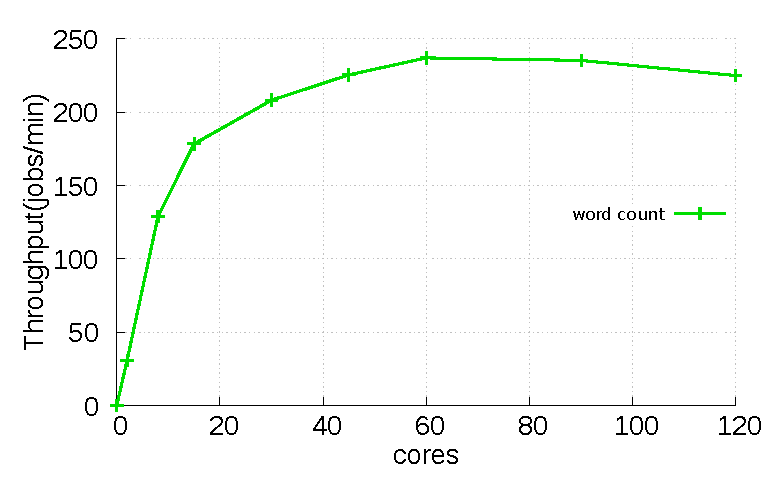
\includegraphics[width=1.8in]{graph/wc.eps}
        \caption{Word Count}
    \end{subfigure}%
    \begin{subfigure}[b]{0.25\textwidth}
        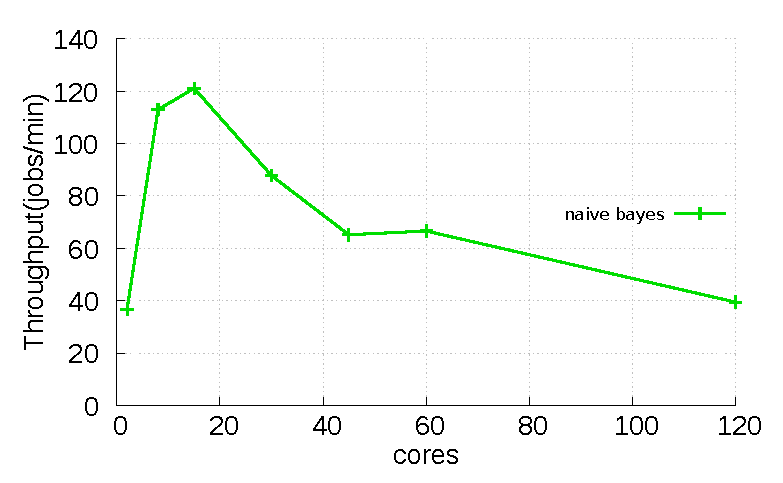
\includegraphics[width=1.8in]{graph/nb.eps}
        \caption{Naive Basian}
    \end{subfigure}%
    \begin{subfigure}[b]{0.25\textwidth}
        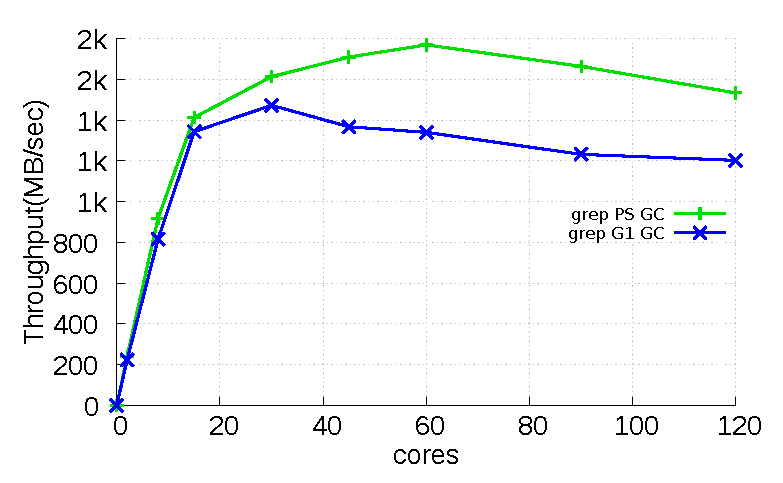
\includegraphics[width=1.8in]{graph/grep.eps}
        \caption{Grep}
    \end{subfigure}%
    \begin{subfigure}[b]{0.25\textwidth}
        \includegraphics[width=1.8in]{graph/kmeans.eps}
        \caption{K-means}
    \end{subfigure}%
    \caption{Performance scalability.}
    \label{fig:scalability}
\end{figure*}



\begin{figure*}[tb]
    \centering
    \begin{subfigure}[b]{0.25\textwidth}
        \includegraphics[width=1.8in]{graph/wc_cpuutils.eps}
        \caption{Word Count}
    \end{subfigure}%
    \begin{subfigure}[b]{0.25\textwidth}
        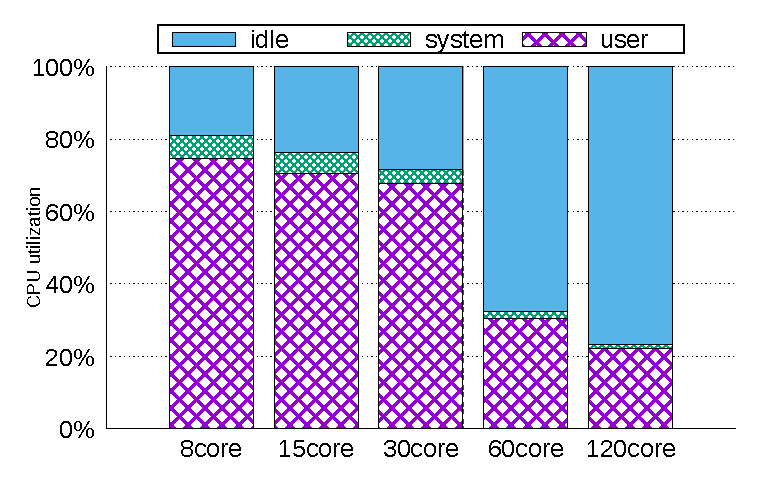
\includegraphics[width=1.8in]{graph/nb_cpuutils.eps}
        \caption{Naive Basian}
    \end{subfigure}%
    \begin{subfigure}[b]{0.25\textwidth}
        \includegraphics[width=1.8in]{graph/grep_cpuutils.eps}
        \caption{Grep}
    \end{subfigure}%
    \begin{subfigure}[b]{0.25\textwidth}
        \includegraphics[width=1.8in]{graph/kmeans_cpuutils.eps}
        \caption{K-means}
    \end{subfigure}%
        \centering
    \caption{CPU utilization.}
    \label{fig:cpuutilization}
\end{figure*}

%$$$$$$$$$$$$$$$$$$$$$$$$$$$$$$$$$$$$$$$$$$$$$$$$$$$$$$$$$$$$$$$$$$$$$$$$$$$$$$$$
%$$$$$$$$$$$$$$$$$$$$$$$$$$$$$$$$$$$$$$$$$$$$$$$$$$$$$$$$$$$$$$$$$$$$$$$$$$$$$$$$
%Mapping
%$$$$$$$$$$$$$$$$$$$$$$$$$$$$$$$$$$$$$$$$$$$$$$$$$$$$$$$$$$$$$$$$$$$$$$$$$$$$$$$$
The rest of this paper is organized as follows.
Section 2 describes the test-bed, Spark scalability problem and benefits of partitioning.
Section 3 shows the our proof-of-concept architecture.
Section 4 describes related works. 
Finally, section 5 concludes the paper.


\section{Scale-up Server Scalalbility}

%$$$$$$$$$$$$$$$$$$$$$$$$$$$$$$$$$$$$$$$$$$$$$$$$$$$$$$$$$$$$$$$$$$$$$$$$$$$$$$$$
%$$$$$$$$$$$$$$$$$$$$$$$$$$$$$$$$$$$$$$$$$$$$$$$$$$$$$$$$$$$$$$$$$$$$$$$$$$$$$$$$
% Apache Spark에 대한 설명
%$$$$$$$$$$$$$$$$$$$$$$$$$$$$$$$$$$$$$$$$$$$$$$$$$$$$$$$$$$$$$$$$$$$$$$$$$$$$$$$$

\ifkor
이번 장에서는 스파크의 Scalalbility에 대해서 설명한다.
\else

\fi

%$$$$$$$$$$$$$$$$$$$$$$$$$$$$$$$$$$$$$$$$$$$$$$$$$$$$$$$$$$$$$$$$$$$$$$$$$$$$$$$$
%$$$$$$$$$$$$$$$$$$$$$$$$$$$$$$$$$$$$$$$$$$$$$$$$$$$$$$$$$$$$$$$$$$$$$$$$$$$$$$$$
% 이번 장에 대한 설명
%$$$$$$$$$$$$$$$$$$$$$$$$$$$$$$$$$$$$$$$$$$$$$$$$$$$$$$$$$$$$$$$$$$$$$$$$$$$$$$$$
\ifkor
벤치마크는 BigData Benchmark를 사용하였다.
\else

\fi

\subsection{Test-Bed and Benchmark}

%$$$$$$$$$$$$$$$$$$$$$$$$$$$$$$$$$$$$$$$$$$$$$$$$$$$$$$$$$$$$$$$$$$$$$$$$$$$$$$$$
%$$$$$$$$$$$$$$$$$$$$$$$$$$$$$$$$$$$$$$$$$$$$$$$$$$$$$$$$$$$$$$$$$$$$$$$$$$$$$$$$
% 테스트 베드 설명
%$$$$$$$$$$$$$$$$$$$$$$$$$$$$$$$$$$$$$$$$$$$$$$$$$$$$$$$$$$$$$$$$$$$$$$$$$$$$$$$$
\ifkor
IBM server에 대한 설명 
\else

\fi


%$$$$$$$$$$$$$$$$$$$$$$$$$$$$$$$$$$$$$$$$$$$$$$$$$$$$$$$$$$$$$$$$$$$$$$$$$$$$$$$$
%$$$$$$$$$$$$$$$$$$$$$$$$$$$$$$$$$$$$$$$$$$$$$$$$$$$$$$$$$$$$$$$$$$$$$$$$$$$$$$$$
%Benchamrk에 대한 설명
%$$$$$$$$$$$$$$$$$$$$$$$$$$$$$$$$$$$$$$$$$$$$$$$$$$$$$$$$$$$$$$$$$$$$$$$$$$$$$$$$
\ifkor
벤치마크와 워크로드에 대한 BigData Benchmark를 사용하였다.
\else

\fi

\subsection{Spark Scalability Problem}


\begin{figure*}[tb]
    \centering
    \begin{subfigure}[b]{0.33\textwidth}
        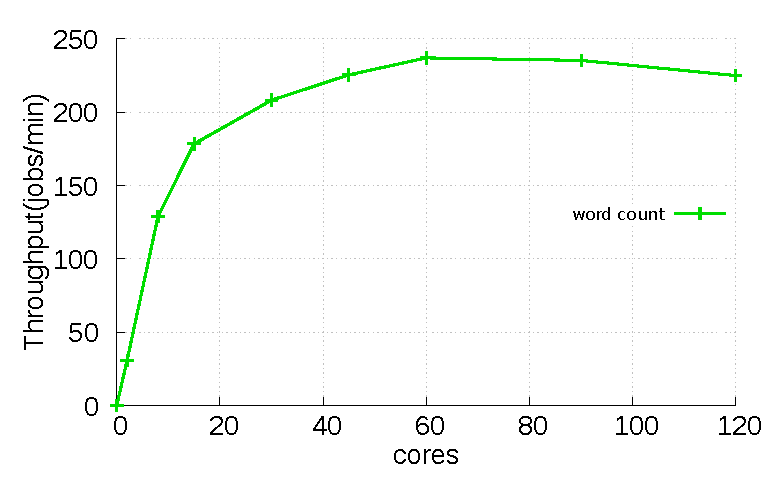
\includegraphics[width=2.2in]{graph/wc.eps}
        \caption{Word Count}
    \end{subfigure}%
    \begin{subfigure}[b]{0.33\textwidth}
        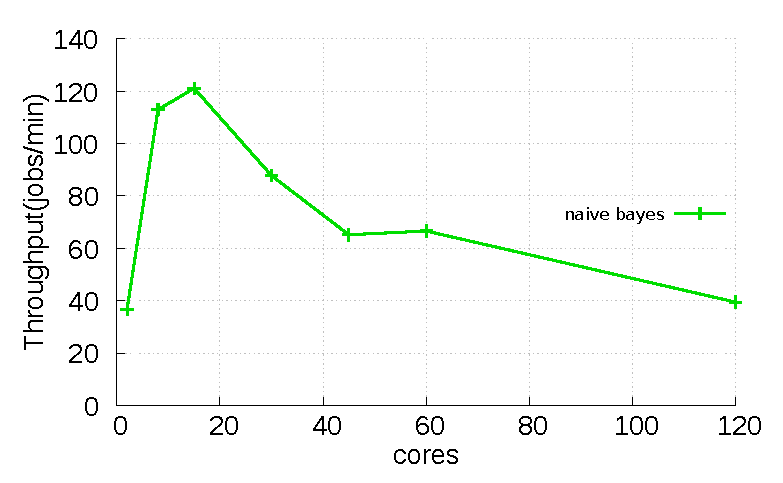
\includegraphics[width=2.2in]{graph/nb.eps}
        \caption{Naive Basian}
    \end{subfigure}%
    \begin{subfigure}[b]{0.33\textwidth}
        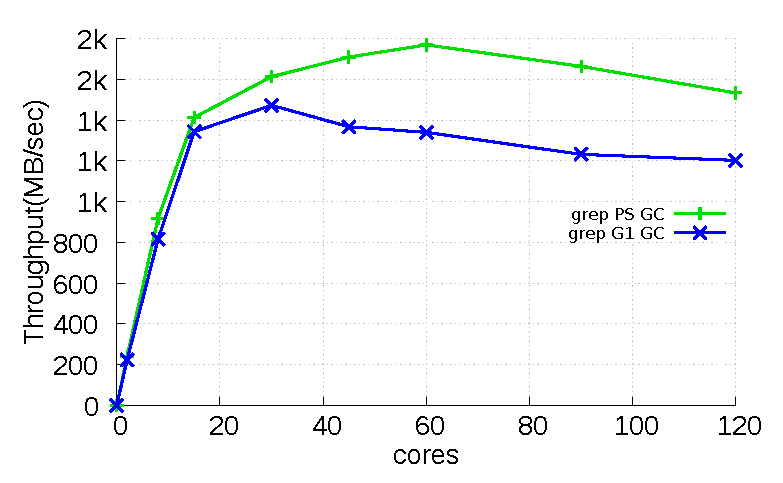
\includegraphics[width=2.2in]{graph/grep.eps}
        \caption{Grep}
    \end{subfigure}
        \begin{subfigure}[b]{0.33\textwidth}
        \includegraphics[width=2.2in]{graph/pagerank.eps}
        \caption{Pagerank}
    \end{subfigure}%
     \begin{subfigure}[b]{0.33\textwidth}
        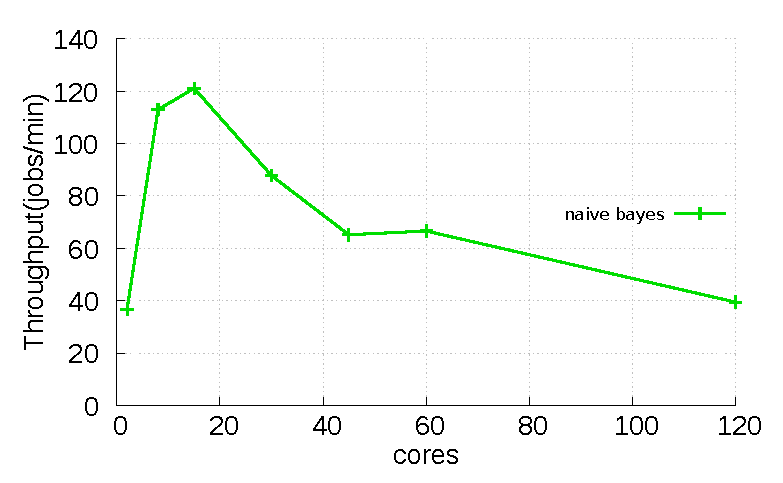
\includegraphics[width=2.2in]{graph/nb.eps}
        \caption{Naive Basian}
    \end{subfigure}%
    \begin{subfigure}[b]{0.33\textwidth}
        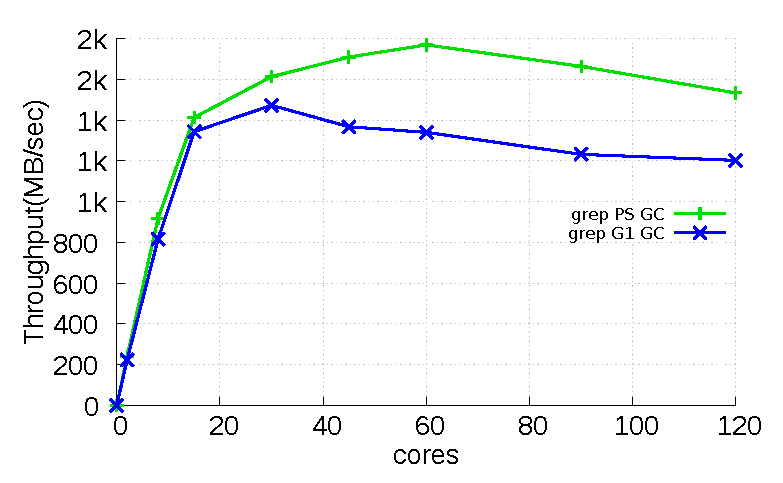
\includegraphics[width=2.2in]{graph/grep.eps}
        \caption{Grep}
    \end{subfigure}
    
        \centering
    \caption{CPU utilization on 120 core.}
    \label{fig:utilization}
\end{figure*}


%$$$$$$$$$$$$$$$$$$$$$$$$$$$$$$$$$$$$$$$$$$$$$$$$$$$$$$$$$$$$$$$$$$$$$$$$$$$$$$$$
%$$$$$$$$$$$$$$$$$$$$$$$$$$$$$$$$$$$$$$$$$$$$$$$$$$$$$$$$$$$$$$$$$$$$$$$$$$$$$$$$
%Scalability 결과에 대한 설명
%$$$$$$$$$$$$$$$$$$$$$$$$$$$$$$$$$$$$$$$$$$$$$$$$$$$$$$$$$$$$$$$$$$$$$$$$$$$$$$$$


\begin{figure*}[tb]
    \centering
    \begin{subfigure}[b]{0.25\textwidth}
        \includegraphics[width=1.8in]{graph/wc_cpuutils.eps}
        \caption{Word Count}
    \end{subfigure}%
    \begin{subfigure}[b]{0.25\textwidth}
        \includegraphics[width=1.8in]{graph/wc_cpuutils.eps}
        \caption{Naive Basian}
    \end{subfigure}%
    \begin{subfigure}[b]{0.25\textwidth}
        \includegraphics[width=1.8in]{graph/wc_cpuutils.eps}
        \caption{Grep}
    \end{subfigure}%
        \begin{subfigure}[b]{0.25\textwidth}
        \includegraphics[width=1.8in]{graph/wc_cpuutils.eps}
        \caption{Pagerank}
    \end{subfigure}
        \centering
    \caption{CPU utilization on 120 core.}
    \label{fig:utilization}
\end{figure*}
Figure~\ref{fig:utilization}(a)) since it waits to acquire

\ifkor
벤치마크와 워크로드에 대한 BigData Benchmark를 사용하였다.
\else

\fi


%$$$$$$$$$$$$$$$$$$$$$$$$$$$$$$$$$$$$$$$$$$$$$$$$$$$$$$$$$$$$$$$$$$$$$$$$$$$$$$$$
%$$$$$$$$$$$$$$$$$$$$$$$$$$$$$$$$$$$$$$$$$$$$$$$$$$$$$$$$$$$$$$$$$$$$$$$$$$$$$$$$
%Lock에 대한 설명
%$$$$$$$$$$$$$$$$$$$$$$$$$$$$$$$$$$$$$$$$$$$$$$$$$$$$$$$$$$$$$$$$$$$$$$$$$$$$$$$$

\ifkor
벤치마크와 워크로드에 대한 BigData Benchmark를 사용하였다.
\else

\fi



%$$$$$$$$$$$$$$$$$$$$$$$$$$$$$$$$$$$$$$$$$$$$$$$$$$$$$$$$$$$$$$$$$$$$$$$$$$$$$$$$
%$$$$$$$$$$$$$$$$$$$$$$$$$$$$$$$$$$$$$$$$$$$$$$$$$$$$$$$$$$$$$$$$$$$$$$$$$$$$$$$$
%Perf에 대한 설명
%$$$$$$$$$$$$$$$$$$$$$$$$$$$$$$$$$$$$$$$$$$$$$$$$$$$$$$$$$$$$$$$$$$$$$$$$$$$$$$$$

\ifkor
벤치마크와 워크로드에 대한 BigData Benchmark를 사용하였다.
\else

\fi





\section{Partitioning for Spark}
%$$$$$$$$$$$$$$$$$$$$$$$$$$$$$$$$$$$$$$$$$$$$$$$$$$$$$$$$$$$$$$$$$$$$$$$$$$$$$$$$
%$$$$$$$$$$$$$$$$$$$$$$$$$$$$$$$$$$$$$$$$$$$$$$$$$$$$$$$$$$$$$$$$$$$$$$$$$$$$$$$$
% 일반적인 매니코어 또는 Scale-server의 scalability 대한 설명과 이번장에 대한 설명
%$$$$$$$$$$$$$$$$$$$$$$$$$$$$$$$$$$$$$$$$$$$$$$$$$$$$$$$$$$$$$$$$$$$$$$$$$$$$$$$$
\ifkor
파티션닝 방법이 필요한 이유는 spark library와 runtime엔진이 single node에 동작하는 
시스템의 scalability 특성을 고려하지 않았기 때문이다. 
scale-up server를 위한 spark scalability의 근본적인 해결 방법은 spark library와 
runtime엔진을 scale-up서버를 위해 scalable하게 만드는 것이다.
하지만 scale-out 시스템의 scalability를 위해 작성된 spark의 library와 runtime 엔진을 
수정하는것은 쉽지않다.
이러한 single node로 구성된 manycore scale-up 서버에 대한 scalability
문제는 도커를 활용한 파티셔닝 기법을 사용하여 해결할 수 있다.
이번 장에서는 우리가 수행한 파티션닝 방법이 필요한 이유와 우리가 수행한 방법에 대해서 설명한다.
\else

\fi

%$$$$$$$$$$$$$$$$$$$$$$$$$$$$$$$$$$$$$$$$$$$$$$$$$$$$$$$$$$$$$$$$$$$$$$$$$$$$$$$$
%$$$$$$$$$$$$$$$$$$$$$$$$$$$$$$$$$$$$$$$$$$$$$$$$$$$$$$$$$$$$$$$$$$$$$$$$$$$$$$$$
% NUMA 영향에 대한 설명
%$$$$$$$$$$$$$$$$$$$$$$$$$$$$$$$$$$$$$$$$$$$$$$$$$$$$$$$$$$$$$$$$$$$$$$$$$$$$$$$$
\ifkor
파티션닝 방법이 필요한 가장 큰 이유는 DRAM access latency 때문이다. 
만약 scale-up server가 NUMA 아키텍쳐를 가진 경우일 경우, 
리눅스는 이러한 문제를 해결하기 위해 커널 내부에 automatic NUMA balancing이라는 기능이 있으나, 
아직 파티션되어 수행하는 방법보다는 성능이 떨어진다[]. 그림 xx-xx는 NUMA balancing을 
사용한 방법과 파티션기법을 사용한 방법의 성능 측정한 결과를 보여준다. 
\else

\fi

%$$$$$$$$$$$$$$$$$$$$$$$$$$$$$$$$$$$$$$$$$$$$$$$$$$$$$$$$$$$$$$$$$$$$$$$$$$$$$$$$
%$$$$$$$$$$$$$$$$$$$$$$$$$$$$$$$$$$$$$$$$$$$$$$$$$$$$$$$$$$$$$$$$$$$$$$$$$$$$$$$$
% Linux kernel scalability (lock, cache cohearnci, scheduler)등등 OS 노이즈에 대한 설명
%$$$$$$$$$$$$$$$$$$$$$$$$$$$$$$$$$$$$$$$$$$$$$$$$$$$$$$$$$$$$$$$$$$$$$$$$$$$$$$$$
\ifkor
NUMA의 영향 뿐만 아니라, operating system의 scalability 저해 요소 때문에 파티션닝 방법은 필요하다.
Shared memory 시스템의 공유데이터 때문에 발생하는 scalability 저해 요소 때문에 필요하다.
첫째로 공유 데이터를 lock이 있다. 표 xxx 앞에서 실험한 spark의 wordcount에 대해서 .
JVM 위에서 동작하는 thread간의 공유하는 single address space때문에 발생하는 공유 문제이다.
다음으로 scheduler가 아직 
마지막으로 cache cohearci traffic이 있다. 

\else

\fi

%$$$$$$$$$$$$$$$$$$$$$$$$$$$$$$$$$$$$$$$$$$$$$$$$$$$$$$$$$$$$$$$$$$$$$$$$$$$$$$$$
%$$$$$$$$$$$$$$$$$$$$$$$$$$$$$$$$$$$$$$$$$$$$$$$$$$$$$$$$$$$$$$$$$$$$$$$$$$$$$$$$
% 스파크는 결국 : shared memory system -> distributed system 처럼해야한다. 
%$$$$$$$$$$$$$$$$$$$$$$$$$$$$$$$$$$$$$$$$$$$$$$$$$$$$$$$$$$$$$$$$$$$$$$$$$$$$$$$$
\ifkor
이처럼 NUMA와 shared memory의 공유 데이터 때문에 발생하는 scalability 저해 요소 때문에, 
scale-up 서버를 위한 스파크도 distributed system의 개념처럼 동작해야한다.
따라서 본 연구는 메모리와 CPU를 파티션닝을 하여 마치 shared memory 시스템을 distributed system 
처럼 동작하도록 제안 한다.
스마크 워커들은 모두 독립적인 cpu와 memory를 할당받아 최대한 thread간의 공유메모리와 remote
memory에 접근을 막도록 하였다.
\else

\fi

\begin{figure}[h]
  \begin{center}
     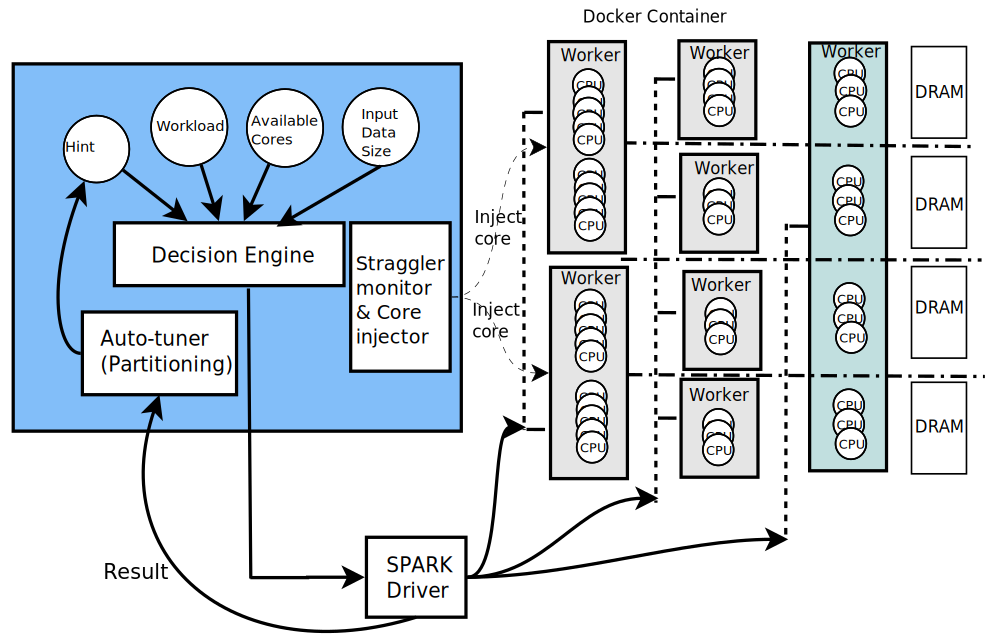
\includegraphics[width=0.5\textwidth]{fig/jaildocker}
  \end{center}
  \caption{The example showing seven update operations(insert C, insert D ,
  reader executes with lock.}
  \label{fig:basic}
\end{figure}


%$$$$$$$$$$$$$$$$$$$$$$$$$$$$$$$$$$$$$$$$$$$$$$$$$$$$$$$$$$$$$$$$$$$$$$$$$$$$$$$$
%$$$$$$$$$$$$$$$$$$$$$$$$$$$$$$$$$$$$$$$$$$$$$$$$$$$$$$$$$$$$$$$$$$$$$$$$$$$$$$$$
% 제안하는 구조 framework 설명
%$$$$$$$$$$$$$$$$$$$$$$$$$$$$$$$$$$$$$$$$$$$$$$$$$$$$$$$$$$$$$$$$$$$$$$$$$$$$$$$$
\ifkor
본 연구에서 제안하는 구조는 그림 <x>와 같다. 
모든 cpu들은 파티션이 되어 동작하며, 모두 스파크 워커로 동작한다.
도커의 파티션은 한 소켓에서 해당하는 cpu 수를 최대로 하여 파티션을 한 후 
계속 코어 수를 줄이며 파티션을 수행한다. 
예를 들어 15코어를 가진 NUMA 노드일 경우, 15코어 단위로 Docker 파티션을 구성 한 후,
(7,8) 와 같이 추가적인 파티션 조합으로 구성한다.
이러한 파티션은 
가장 최적의 방법은 best fit을 찾는 과정이 필요하다. 
\else

\fi


%$$$$$$$$$$$$$$$$$$$$$$$$$$$$$$$$$$$$$$$$$$$$$$$$$$$$$$$$$$$$$$$$$$$$$$$$$$$$$$$$
%$$$$$$$$$$$$$$$$$$$$$$$$$$$$$$$$$$$$$$$$$$$$$$$$$$$$$$$$$$$$$$$$$$$$$$$$$$$$$$$$
% Docker를 이용하는 이유
%$$$$$$$$$$$$$$$$$$$$$$$$$$$$$$$$$$$$$$$$$$$$$$$$$$$$$$$$$$$$$$$$$$$$$$$$$$$$$$$$
\ifkor
우리는 Worker들의 파티션닝을 위해 Docker container를 사용하였다. 
그 이유는 virtual machine보다 훨씬 가벼운 구조로 되어 있으며, 
최근 docker기반으로 시스템을 관리하는 구조로 변경되고 있기 때문이다.
예를 들어 google kubernet을 사용할 경우, 워크마다 가장 최적의 파티션닝 값을 구한 후
그에 맞는 도커 컨테이너를 실행시키는 방법으로 구성하면 된다.
따라서 본 연구의 파티셔닝을 위한 방법으로 Docker container를 사용하였다.
\else

\fi


The basic principle of update-side absorbing is that update uses atomic 
marking operation for the object's mark field, which allows previous operation to cancel.
For instance, if a new remove operation occurs after insert operation of the
same object, deferu does not store this operation in the lock-less
list; instead, it changes the insert mark field to zero using the CAS.
This mark is checked later when reading operation occurs and the operation log 
maintained in the lock-less list is applied to original data structure atomically.




%$$$$$$$$$$$$$$$$$$$$$$$$$$$$$$$$$$$$$$$$$$$$$$$$$$$$$$$$$$$$$$$$$$$$$$$$$$$$$$$$
%$$$$$$$$$$$$$$$$$$$$$$$$$$$$$$$$$$$$$$$$$$$$$$$$$$$$$$$$$$$$$$$$$$$$$$$$$$$$$$$$
% Linux kernel scalability (lock, cache cohearnci, scheduler)등등 OS 노이즈에 대한 설명
%$$$$$$$$$$$$$$$$$$$$$$$$$$$$$$$$$$$$$$$$$$$$$$$$$$$$$$$$$$$$$$$$$$$$$$$$$$$$$$$$
\ifkor
NUMA의 영향 뿐만 아니라, operating system의 scalability 저해 요소 때문에 파티션닝 방법은 필요하다.
Shared memory 시스템의 공유데이터 때문에 발생하는 scalability 저해 요소 때문에 필요하다.
첫째로 공유 데이터를 lock이 있다. 표 xxx 앞에서 실험한 spark의 wordcount에 대해서 .
JVM 위에서 동작하는 thread간의 공유하는 single address space때문에 발생하는 공유 문제이다.
다음으로 scheduler가 아직 
마지막으로 cache cohearci traffic이 있다. 

\else

\fi



\section{Evaluation}


\begin{figure*}[tb]
    \centering
    \begin{subfigure}[b]{0.33\textwidth}
        \includegraphics[width=2.2in]{graph/wc_docker.eps}
        \caption{Exim - 120core}
    \end{subfigure}%
    \begin{subfigure}[b]{0.33\textwidth}
        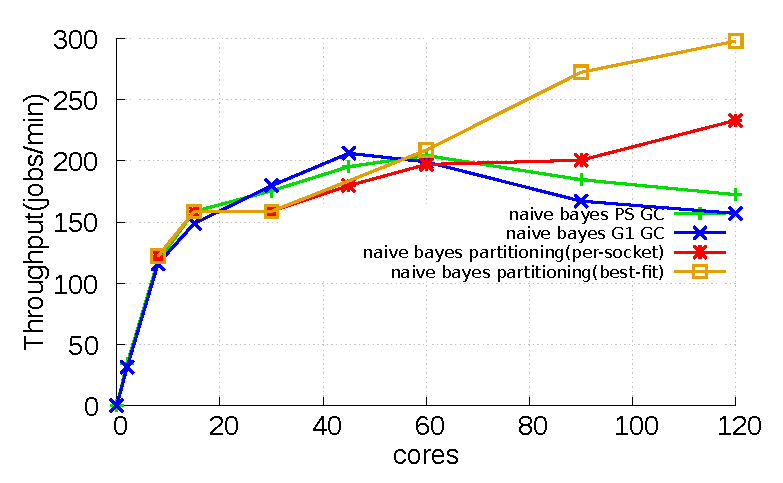
\includegraphics[width=2.2in]{graph/nb_docker.eps}
        \caption{Lmbench - 120core}
    \end{subfigure}%
    \begin{subfigure}[b]{0.33\textwidth}
        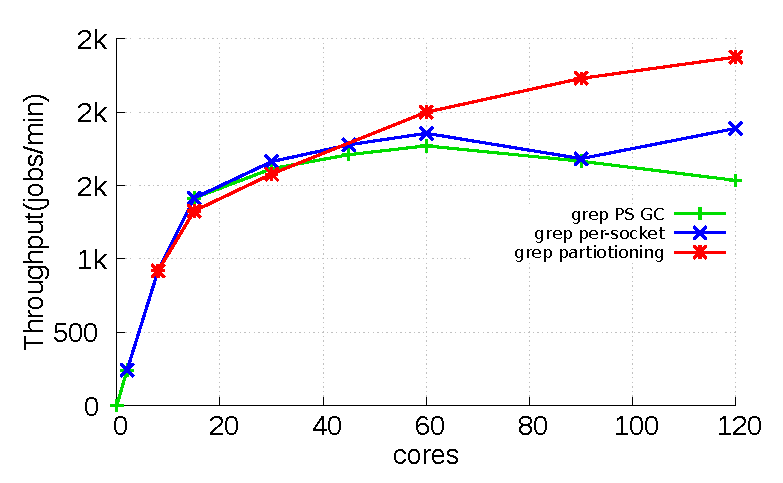
\includegraphics[width=2.2in]{graph/grep_docker.eps}
        \caption{AIM7 - 120core}
    \end{subfigure}
        \begin{subfigure}[b]{0.33\textwidth}
        \includegraphics[width=2.2in]{graph/pagerank_docker.eps}
        \caption{Lmbench - 120core}
    \end{subfigure}%
        \begin{subfigure}[b]{0.33\textwidth}
        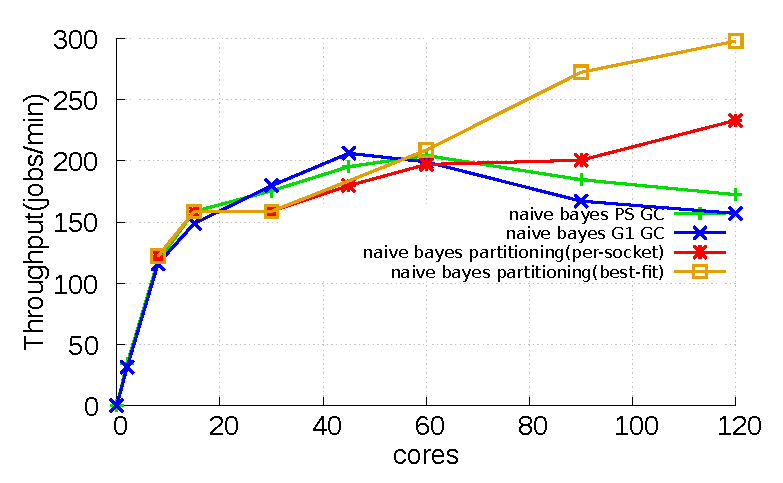
\includegraphics[width=2.2in]{graph/nb_docker.eps}
        \caption{Lmbench - 120core}
    \end{subfigure}%
    \begin{subfigure}[b]{0.33\textwidth}
        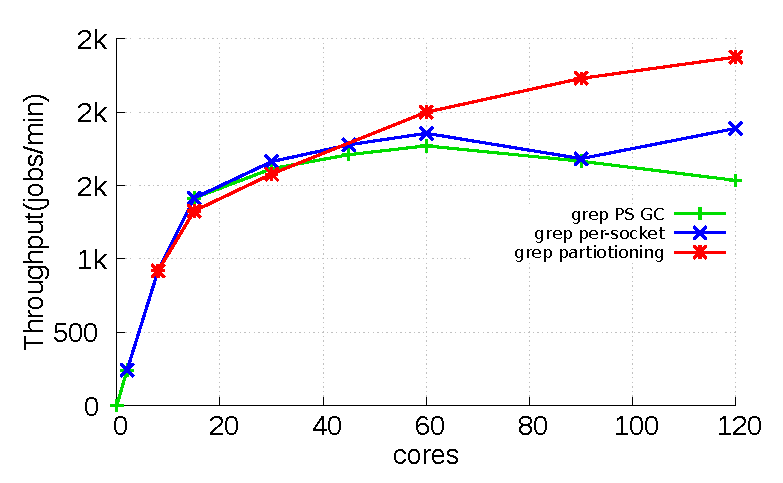
\includegraphics[width=2.2in]{graph/grep_docker.eps}
        \caption{AIM7 - 120core}
    \end{subfigure}
        \centering
    \caption{CPU utilization on 120 core.}
    \label{fig:utilization3}
\end{figure*}



\begin{figure*}[tb]
    \centering
    \begin{subfigure}[b]{0.25\textwidth}
        \includegraphics[width=1.8in]{graph/wc_cpuutils.eps}
        \caption{Word Count}
    \end{subfigure}%
    \begin{subfigure}[b]{0.25\textwidth}
        \includegraphics[width=1.8in]{graph/wc_cpuutils.eps}
        \caption{Naive Basian}
    \end{subfigure}%
    \begin{subfigure}[b]{0.25\textwidth}
        \includegraphics[width=1.8in]{graph/wc_cpuutils.eps}
        \caption{Grep}
    \end{subfigure}%
        \begin{subfigure}[b]{0.25\textwidth}
        \includegraphics[width=1.8in]{graph/wc_cpuutils.eps}
        \caption{Pagerank}
    \end{subfigure}
        \centering
    \caption{CPU utilization on 120 core.}
    \label{fig:utilization2}
\end{figure*}


%$$$$$$$$$$$$$$$$$$$$$$$$$$$$$$$$$$$$$$$$$$$$$$$$$$$$$$$$$$$$$$$$$$$$$$$$$$$$$$$$
%Paragraph 1: 실험 환경 설명
%$$$$$$$$$$$$$$$$$$$$$$$$$$$$$$$$$$$$$$$$$$$$$$$$$$$$$$$$$$$$$$$$$$$$$$$$$$$$$$$$
\ifkor
이번 장에서는 스파크의 Scalalbility에 대해서 설명한다.
\else

\fi




%$$$$$$$$$$$$$$$$$$$$$$$$$$$$$$$$$$$$$$$$$$$$$$$$$$$$$$$$$$$$$$$$$$$$$$$$$$$$$$$$
%Paragraph 2: 비교 대상 설명
%$$$$$$$$$$$$$$$$$$$$$$$$$$$$$$$$$$$$$$$$$$$$$$$$$$$$$$$$$$$$$$$$$$$$$$$$$$$$$$$$
\ifkor
이번 장에서는 스파크의 Scalalbility에 대해서 설명한다.
\else

\fi




%$$$$$$$$$$$$$$$$$$$$$$$$$$$$$$$$$$$$$$$$$$$$$$$$$$$$$$$$$$$$$$$$$$$$$$$$$$$$$$$$
%Paragraph 2: A그룹에 대한 실험 결
%$$$$$$$$$$$$$$$$$$$$$$$$$$$$$$$$$$$$$$$$$$$$$$$$$$$$$$$$$$$$$$$$$$$$$$$$$$$$$$$$
\ifkor
이번 장에서는 스파크의 Scalalbility에 대해서 설명한다.
\else

\fi




%$$$$$$$$$$$$$$$$$$$$$$$$$$$$$$$$$$$$$$$$$$$$$$$$$$$$$$$$$$$$$$$$$$$$$$$$$$$$$$$$
%Paragraph 2: b그룹에 대한 실험 결
%$$$$$$$$$$$$$$$$$$$$$$$$$$$$$$$$$$$$$$$$$$$$$$$$$$$$$$$$$$$$$$$$$$$$$$$$$$$$$$$$
\ifkor
이번 장에서는 스파크의 Scalalbility에 대해서 설명한다.
\else

\fi



%$$$$$$$$$$$$$$$$$$$$$$$$$$$$$$$$$$$$$$$$$$$$$$$$$$$$$$$$$$$$$$$$$$$$$$$$$$$$$$$$
%Paragraph 2: CPU utilization에 대한 설명
%$$$$$$$$$$$$$$$$$$$$$$$$$$$$$$$$$$$$$$$$$$$$$$$$$$$$$$$$$$$$$$$$$$$$$$$$$$$$$$$$
\ifkor
이번 장에서는 스파크의 Scalalbility에 대해서 설명한다.
\else

\fi

\section{Related work} \label{sec:RelatedWork}

%$$$$$$$$$$$$$$$$$$$$$$$$$$$$$$$$$$$$$$$$$$$$$$$$$$$$$$$$$$$$$$$$$$$$$$$$$$$$$$$$
%Paragraph 1:Linux Scalability의 연구에 대한 설명
%$$$$$$$$$$$$$$$$$$$$$$$$$$$$$$$$$$$$$$$$$$$$$$$$$$$$$$$$$$$$$$$$$$$$$$$$$$$$$$$$
\ifkor
\noindent
\textbf{Apache Spark Scalability.}
To improve the scalability, researchers have attempted to create new
operating systems~\cite{Boyd-WickizerCorey}~\cite{Wentzlaff2010fOS}
%~\cite{Baumann2009Barrelfish}~\cite{Zellweger2014Multikernel}
%~\cite{Liu2009Tessellation}~\cite{Farrington2010Helios}
or have
attempted to optimize existing operating systems~\cite{SilasBoydWickizer2010LinuxScales48}~\cite{AustinTClements2012RCUBalancedTrees}~\cite{Clements2013RadixVM}~\cite{SilasBoydWickizerPth}
%~\cite{Changwoo2016UMSF}.
Our research belongs to optimizing existing operating systems in order to
solve the Linux fork scalability problem.
However, previous research did not deal with the anonymous reverse mapping,
which is one of the fork scalability bottleneck.

\else

\fi

%$$$$$$$$$$$$$$$$$$$$$$$$$$$$$$$$$$$$$$$$$$$$$$$$$$$$$$$$$$$$$$$$$$$$$$$$$$$$$$$$
%Paragraph 1:Manycore Scalability의 연구에 대한 설명
%$$$$$$$$$$$$$$$$$$$$$$$$$$$$$$$$$$$$$$$$$$$$$$$$$$$$$$$$$$$$$$$$$$$$$$$$$$$$$$$$
\ifkor
\noindent
\textbf{Manycore Scalability.}
OS scalability.원천기술.
Scalable locks have been designed by the
queue-based locks~\cite{MellorCrummey1991MCS}~\cite{Magnusson1994QLC},
%~\cite{Wang2016BeMyGuest},
%~\cite{Scott2013SS}
%~\cite{Bueso2014MCS}~\cite{Bueso2015STP}
hierarchical locks~\cite{Radovic2003HBL}~\cite{Chabbi2016CLL} and
%~\cite{Luchangco2006HCQ}
%~\cite{Chabbi2015HPL}
delegation techniques~\cite{Hendler2010FC}~\cite{Fatourou2012RCS}~\cite{Delegation2014}.
%Some approaches have been gradually adapted in real production software.
%For example, Linux kernel has replaced non-scalable locks with
%MCS locks~\cite{overviewofkernellock}.
Our research is similar to the delegation techniques because
the s \code{synchronize} function runs as a
combiner thread;it improves cache locality.
However, our approach not only can improve cache locality but also
can eliminate synchronization methods during updates due to using a lock-free manner.
%MCS~\cite{MellorCrummey91}, a scalable lock.

\else

\fi

%$$$$$$$$$$$$$$$$$$$$$$$$$$$$$$$$$$$$$$$$$$$$$$$$$$$$$$$$$$$$$$$$$$$$$$$$$$$$$$$$
%Paragraph 1:Manycore Partitioning의 연구에 대한 설명
%$$$$$$$$$$$$$$$$$$$$$$$$$$$$$$$$$$$$$$$$$$$$$$$$$$$$$$$$$$$$$$$$$$$$$$$$$$$$$$$$
\ifkor
\noindent
\textbf{Manycore Partitioning.}
In order to improve Li
멀티커널.등등 공유메모리를 사용 X
Many scalable data structures with scalable schemes show
different performances depending on their update ratios.
In low and middle update rate, researchers have attempted to create new scalable
schemes~\cite{McKenney98}~\cite{Matveev2015RLU}~\cite{Harris2001Lockfree}
%~\cite{Fomitchev2004Lockfree}
%~\cite{Timnat2012}
or have attempted to adapt these scheme to data structures~\cite{Arbel2014ConcurrentRCU}~\cite{Dodds2015SCT}~\cite{AustinTClements2012RCUBalancedTrees}.
In high update rate, the OpLog shows significant improvement in
performance scalability for update-heavy data structures in
many core systems, but suffers from limitation and overhead due
to time-stamp counter management.
We substantially extend our preliminary work~\cite{Kyong2016LDU} not only to support 
per-core algorithm but also to apply the  to anonymous rmap due to improving the
Linux kernel scalability.
\else

\fi



\section{Conclusion and Future Works}

%$$$$$$$$$$$$$$$$$$$$$$$$$$$$$$$$$$$$$$$$$$$$$$$$$$$$$$$$$$$$$$$$$$$$$$$$$$$$$$$$
%Paragraph 1:Spark Scalability의 연구에 대한 설명
%$$$$$$$$$$$$$$$$$$$$$$$$$$$$$$$$$$$$$$$$$$$$$$$$$$$$$$$$$$$$$$$$$$$$$$$$$$$$$$$$
\ifkor
We proposed a docker container-based partitioning method for Apache
Spark scalability on scale-up server.
To eliminate GC and remote memory access, we divided per-socket and best-fit partitioning
using the docker container.
Evaluation results(Word Count, Naive Basian, Grep and K-means) reveal
that our method has substantial performance up to 1.7 times compared to existing
solutions.
\newline\\
\noindent
\textbf{Future Directions.} Our future directions are:
\begin{itemize}
\item \textbf{Solving the straggler tasks problem.} straggler tasks
significantly extend job completion times.
To mitigate this problem, we may use dynamic resource allocation solution in
dockers to maximized cpu utilization for the straggler tasks by using our new
resource hand-over solution.
\item \textbf{Implementing the auto-tuner.} In this paper, only support manually
partitioning method. However, many of science applications or big data analytics 
may reuse similar workloads, so training phase for finding the best-fit
partitioning can be a superior solution in a way similar to compiler-based auto-tuner~\cite{Ansel2014OEF}.

\end{itemize}

\else

\fi


\bibliographystyle{plain}
\bibliography{ref}

\ifkor
\end{CJK}
\fi

% That's all folks!
\end{document}
